\documentclass[journal,12pt,twocolumn]{IEEEtran}
\usepackage[utf8]{inputenc}
\usepackage{amsmath}
\usepackage{graphicx}
\usepackage[english]{babel}
\usepackage{hyperref}
\usepackage{tcolorbox}
\urlstyle{same}
\title{Assignment 7 }
\author{Harshal Verma\\
AI21MTECH02003}
\date{April 2021}
\begin{document}
\maketitle
\section{Prob 6.15}
Problem: Given two independent events A and B such that they are independent and P(A) = 0.3
 and P(B) = 0.6, find.\\
(a) $P(\text{A and B})$\\
(b) $P(\text{A and not B})$\\
(c) $P(\text{A or B} )$\\
(d) $P(\text{neither A nor B})$\\
\\
\\
\\
\textbf{Solution (a): $P(\text{A and B})$}:\\
Two events are independent if:\\ $Pr(A\cap B) = Pr(A)*Pr(B) $
 Given Pr(A) = 0.3 and Pr(B) = 0.6\\
 \begin{align}
     Pr( \text {A and B}) &= Pr(A \cap B) \\
     &= Pr(A)\times Pr(B)\\
     &= 0.3 \times 0.6\\
     &= 0.18
 \end{align}
 
 \textbf{ (b): $P(\text{A and nor B})$}:\\
\begin{align}
    Pr(\text{A and not B}) &= Pr(A \cap B')\\
    &=Pr(A) - Pr(A \cap B)\\
    &= 0.3 -0.18\\
    &=0.12\\
\end{align}

\textbf{ (c): $P(\text{A or B})$}:\\
\begin{align}
    Pr(\text{A or B}) &= Pr(A \cup B')\\
    &=Pr(A) +Pr(B) - Pr(A \cap B)\\
    &= 0.3 +0.6 - 0.18\\
    &=0.72\\
\end{align}

\textbf{ (d): $P(\text{Neither A nor B})$}:\\
\begin{align}
    Pr(\text{neither A nor B}) &=Pr(A' and B')\\
    &=Pr(A' \cup B')\\
    &= 1-Pr(A \cup B)\\
    &=1-0.72\\
    &= 0.28
\end{align}

\begin{figure}[htp]
    \centering
    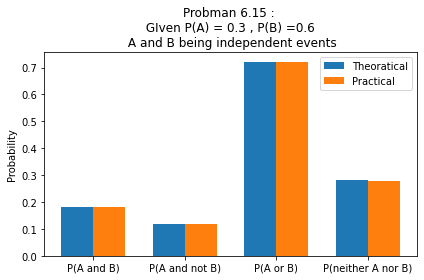
\includegraphics[width=10cm]{Assignment_7}
    \label{fig :plot}
\end{figure}

\begin{tcolorbox}
Code source: \url{https://github.com/harshal9876/AI5002/blob/main/Asssignment_7/Codes/Assignment_7.py} \\
LaTex code :
\url{https://github.com/harshal9876/AI5002/blob/main/Asssignment_7/Assignment_7.tex}
\end{tcolorbox}

\end{document}




